
\vspace{10mm}
\section{Arbitrage free discretization of the Libor Market Model}
\subsection{Definition of {\it arbirtrage-free} discretization}
As it has already been said, in the BGM models it is supposed that all the libor 
$L(t,T_i,\tau)$ under their own foward measure $Q^{T_{i+1}}$  has no drift and 
deterministic log-volatility :
$$\forall i=1,..,M : \quad dL(t,T_i,\tau)=L(t,T_i,\tau)\gamma_i(t).dW^{Q^{T_{i+1}}}_t.$$
Considering a numeraire $N(t)$, we denote by $D_i$ the deflated bonds :
$$\forall i=1,..,M+1 : D_i(t)=\frac{B(t,T_i)}{N(t)}.$$
\noindent {\bf Important remarks :} \\
The
convention for all $i=1,..,M$ : $\forall
t>T_i:\,L(t,T_i,\tau)=L(T_i,T_i,\tau)$ will be necessary which implies
$\gamma_i(t)=0$ for $t \geq T_i$ .  \\
For better understanding, we will denote $u.v$ the scalar product
between 2 vectors and $\lambda * u$ the product between scalar and a
vector.\\
To lighten the notations, when no space intervalle is specified for the
current time $t$ it will mean $for \,all \,t \in [0,T_{M+1}]$.\\
A sum $\sum$ of no term will be $0$ and a product $\prod$ of no term will be $1$.\\

\noindent By definition of a numeraire the deflated bonds are martingale under their 
corresponding measure $Q^N$ associated to the numeraire $N$.
This martingale property is of course for the continuous filtration.\\
The deflated bonds price can be defined by the libors :
$$\forall t<T_i:\quad D_i(t)=\frac{B(t,T_{i_t})}{N(t)}\prod_{j=i_t}^{i-1}\frac{1}{1+\tau
    L(t,T_j,\tau)},\quad \hbox{for } i=i_t,..,M+1$$
where $i_t$ is the unique integer such that $T_{i_t-1} \le t
<T_{i_t}$.\\

\noindent {\bf Definition :} A discretisation $0=t_0<t_1<...<t_n=T_{M+1}$ is said to be
{\it arbitrage-free} if all the discrete deflated bonds are discrete
martingale. In other words, if we denote $\hat{D_i}(t_j)$ the computed
deflated bond $D_i$ in time $t_j$, we must have :
\begin{equation}
\label{def}
\forall i=1,..,M+1, \quad j=0,..,n-1
:\hat{D_i}(t_j)=E\left[\hat{D_i}(t_{j+1}) _{/{F}_j}\right]
\end{equation}
where ${F}_j$ is the filtration  associed to the discrete brownien
process over ${t_0, t_1, ...,t_n}$.\\

\noindent {\bf Remark :} Thus the condition to an {\it arbitrage-free}
discretisation can be resumed to these backward decrete relations.

\subsection{Two usefull numeraires for {\it arbitrage-free}}
There are two numeraires that will be usefull to seek {\it
  arbitrage-free} dicretization.\\
the terminal numeraire :
$$N_T(t)=B(t,T_{M+1})$$
and the spot numraire ($i_t$ such that: $T_{i_t-1} \le t<T_{i_t}$):
$$N_S(t)=\frac{B(t,T_{i_t})}{B(0,T_1) \prod_{j=1}^{i_t-1}B(T_j,T_{j+1})}$$

Both numeraires have the great advantage, for a libor model, to give the
expression of the deflated bonds  only with respect to the libors :
\ba
\label{DtfL}
D_i(t)&=&\prod_{j=i}^{M}\left(1+\tau L(t,T_j,\tau)\right)\quad
\hbox{for the terminal numeraire}\\
\label{DsfL}
D_i(t)&=&B(0,T_1)\prod_{j=1}^{i-1}\frac{1}{1+\tau L(t,T_j,\tau)}\quad
\hbox{for the spot numeraire}
\ea
for all $i=1,...,M+1$.\\
Thus in the {\it libors discrete world}, denoting for all $i=0,..,n$
and $j=1,..,M$
$\hat{L}(t_i,T_j,\tau)$ the numerical computed value of the
libors, the discrete deflated bonds price are: 
\ba
\hat{D}_i(t)&=&\prod_{j=i}^{M}\left(1+\tau \hat{L}(t,T_j,\tau)\right)\quad
\hbox{for the terminal numeraire}\\
\hat{D}_i(t)&=&B(0,T_1)\prod_{j=1}^{i-1}\frac{1}{1+\tau \hat{L}(t,T_j,\tau)}\quad
\hbox{for the spot numeraire}
\ea
\subsection{Continuous martingales versus discrete Martingale}
Martingale property of the continuous deflated bonds does not imply
the martingale property of the discrete deflated bonds. For example in a
BGM model the libors $\hat{L}_i$ or log-libors $log(\hat{L}_i)$ are computed through a standart
Euler scheme then the $\hat{D}_i$ have no (discrete) martingale
property. For other models like HJM over an Euler scheme on the forward
rate, it is possible to chose a consistent drift adjustement to get an {\it
  arbitrage-free} discretisation, but for the libors discretisations no
drift adjusment can be found for such an aim (see \cite{freeGZ}).\\ 
Then other assets associated to the libors by a bijective relation will
be discretized to make the {\it arbitrage-free} discretisation true,
that is to say to make the discrete deflated bonds martingale.

\subsection{Two new  martingale assets}
There are two assets that can be be considered.\\
We denoted them $X$ and $Y$ and they are given by :
\ba
\label{XfL}
X_i(t)&=&L(t,T_i,\tau)\prod_{j=i+1}^{M}\left(1+\tau
  {L}(t,T_j,\tau)\right) \quad \forall i=1,..,M.\\
\label{YfL}
Y_i(t)&=&\tau L(t,T_i,\tau)\prod_{j=1}^{i}\frac{1}{1+\tau
  {L}(t,T_j,\tau)} \quad \forall i=1,..,M.
\ea
Taking $Y_{M+1}(t)=\prod_{j=1}^{M}\frac{1}{1+\tau
  \hat{L}(t,T_j,\tau)}$ we have the following equalities:
\begin{equation}
\sum_{j=1}^{M+1} Y_j(t) = 1.
\end{equation}
The libors can aslo be written with respect to this assets :
\ba
\label{LfX}
L_i(t,T_i,\tau)&=&\frac{X_i(t)}{1+\tau X_{i+1}(t)+..+\tau X_M(t)} \quad \forall i=1,2,..,M.\\
\label{LfY}
L_i(t,T_i,\tau)&=&\frac{Y_i(t)}{\tau (Y_{i+1}(t)+..+Y_{M+1}(t))} \quad \forall i=1,2,..,M.
\ea
The deflated bonds  can also be written with respect to these assets :
\ba
\label{DtfX}
D_i(t)&=&1+\tau \sum_{j=i}^{M}X_j(t) \quad \hbox{for terminal numeraire}\\
\label{DsfY}
D_i(t)&=&B(0,T_1)\sum_{j=i}^{M+1}Y_j(t) \quad \hbox{for spot numeraire}
\ea
and vice versa :
\ba
\label{XfD}
X_i(t)&=&\frac{1}{\tau}(D_i(t)-D_{i+1}(t)) \quad \hbox{for terminal numeraire}\\
\label{YfD}
Y_i(t)&=& \frac{D_i(t)-D_{i+1}(t)}{B(0,T_1)}\quad \hbox{for spot numeraire}
\ea
{\bf Theorem:} The assets $X$ and $Y$ are martingale
respectively under the terminal and spot measure.\\

\noindent {\it Proof :} Since the deflated bonds are martingale by
definition, thanks to (\ref{XfD}) and (\ref{YfD}), it is obvious.\\

\subsection{EDS for assets $X$ and $Y$}
{\bf Theorem:} Under their measure the EDS verified by $X$ and $Y$ are the following~:
\ba
\frac{dX_i(t)}{X_i(t)}&=&\left( \gamma_i(t) + \sum_{j=i+1}^M\frac{\tau 
    X_j(t)*\gamma_j}{1+\tau X_j(t)+...+\tau X_M(t)} \right).dW^{Q^{N_T}} \quad \forall i=1,..,M.\\
\frac{dY_i(t)}{Y_i}&=& \left(\gamma_i
+\sum_{i_t}^{i}\frac{Y_j *\gamma_j}{Y_{j-1}+..+Y_1-1}\right).dW^{Q^{N_S}} \quad
\forall i=1,..,M+1.
\ea
\noindent {\it Proof :} For $dX$, we have under terminal $Q^{N_S}$
$$\frac{dL(t,T_i,\tau)}{L(t,T_i,\tau)}= \gamma_i(t). \left(
  \sum_{j=i+1}^M\frac{\tau L(t,T_j,\tau)*\gamma_j(t) }{1+\tau
  L(t,T_j,\tau)} dt + dW \right)$$
and $$\frac{dL(t,T_M,\tau)}{L(t,T_i,\tau)}=\gamma_M(t) . dW$$
Using these equations to compute $dD$ for the terminal numeraire thanks
  to (\ref{DtfL}) and then using $dD$ to compute $dX$ thanks to
  (\ref{XfD}), we check that indeed the drift of $dD$ is vanishing and
  that the volatility of $X$ is the one in the theorem.\\
Idem for $dY$.\\

\subsection{Implementation of caps and swaptions with $X$ and $Y$}
\noindent{\bf Theorem} With a standart log Euler scheme, the discrete
assets $\hat{X}$ and $\hat{Y}$ are discrete martingales.

\noindent {\it Proof :} The definition relation (\ref{def}) can be checked
quite easyly (see \cite{freeGZ}).\\

\noindent Considering a receiver swaption of a swap rate between $T_\alpha$ and
$T_\beta$ ($\alpha<\beta<M+1$), under the numeraire measure $Q^N$ we
have for its price at time $t=0$ :
\ba
\frac{RS_{\alpha,\beta}}{N(0)}&=&E\left[\frac{1}{N(T_\alpha)}\left(1-B(T_\alpha,T_\beta)-K\sum_{j=\alpha+1}^\beta
    \tau B(T_\alpha,T_j)\right)\right]\\
\label{RS}
\frac{RS_{\alpha,\beta}}{N(0)}&=&E\left[D_\alpha(T_\alpha)-D_\beta(T_\alpha)-K\tau\sum_{j=\alpha+1}^\beta
  D_j(T_\alpha)\right]
\ea
\noindent {\bf Swaption price for asset $X$} :
With equality (\ref{DtfX}) in (\ref{RS}) we get under terminal measure :
\begin{equation}
\frac{RS_{\alpha,\beta}}{B(0,T_{M+1})}=\tau E\left[ \sum_{j=\alpha}^{\beta-1}
  X_j(T_\alpha) - K\tau \sum_{j=\alpha+1}^\beta \left(1+\tau
    \sum_{k=j}^M X_k(T_\alpha)\right)\right]
\end{equation}
\noindent {\bf Swaption price for asset $Y$} :  
With equality (\ref{DsfY}) in (\ref{RS}) we get under spot measure:
\begin{equation}
\frac{RS_{\alpha,\beta}}{N_S(0)}= B(0,T_1)E\left[ \sum_{j=\alpha}^{\beta-1} 
  Y_j(T_\alpha) - K\tau \sum_{j=\alpha+1}^\beta 
    \sum_{k=j}^{M+1} Y_k(T_\alpha)\right]
\end{equation}
\noindent {\bf Caplet price for asset $X$} :
Using (\ref{LfX}) we have for a caplet price over $L(T_i,T_i,\tau)$ under terminal measure :
\begin{equation}
\frac{Caplet_i}{N_T(0)}=E\left[X_i(T_\alpha)\frac{1+\tau \sum_{j=i}^{M}X_j(T_\alpha)}{ 1+\tau \sum_{j=i+1}^{M}X_j(T_\alpha)}-K\left(1+\tau \sum_{j=i}^{M}X_j(T_\alpha)\right)\right]
\end{equation}
\noindent {\bf Caplet price for asset $Y$} :
Using (\ref{LfY}) we have for a caplet price over $L(T_i,T_i,\tau)$ under spot measure :
\begin{equation}
\frac{Caplet_i}{N_S(0)}=B(0,T_1)E\left[Y_i(T_\alpha)\frac{\sum_{j=i}^{M+1}Y_j(T_\alpha)}{\sum_{j=i+1}^{M+1}Y_j(T_\alpha)}-K\left(1+\tau \sum_{j=i}^{M+1}Y_j(T_\alpha)\right)\right]
\end{equation}

\subsection{Simulations results}
The zero coupon bonds can be expressed with an expectation. We have
$$B(0,T_i)=N(0)\frac{B(0,T_i)}{N(0)}=N(0)E(D_i(T_i)).$$
Thanks to the exact martingale property of the discrete deflated
bonds $\hat{D}_i$ we can say that if we compute the expectation of the
previous formula, the error only comes from noises due to the number of
Monte-Carlo draws and will tend to vanish when this number goes to
infinity. See the next figures (\ref{bonderrorX}) and  (\ref{bonderrorY}) .
\begin{figure}[H]
\begin{center}
\includegraphics[height=8cm]{./figures/bondserror.eps}
\caption{Cumputation bonds error with martingale asset X for $10 000$, $100 000$ and $1 000 000$ Monte-carlo
  draws, for $\tau=0.25$ and $M=28$ (Number of factor=$1$, $\gamma_i=0.15$ and $L(0,T_i,T_i)=0.05$).}
\label{bonderrorX}
\end{center}
\end{figure}

\begin{figure}[H]
\begin{center}
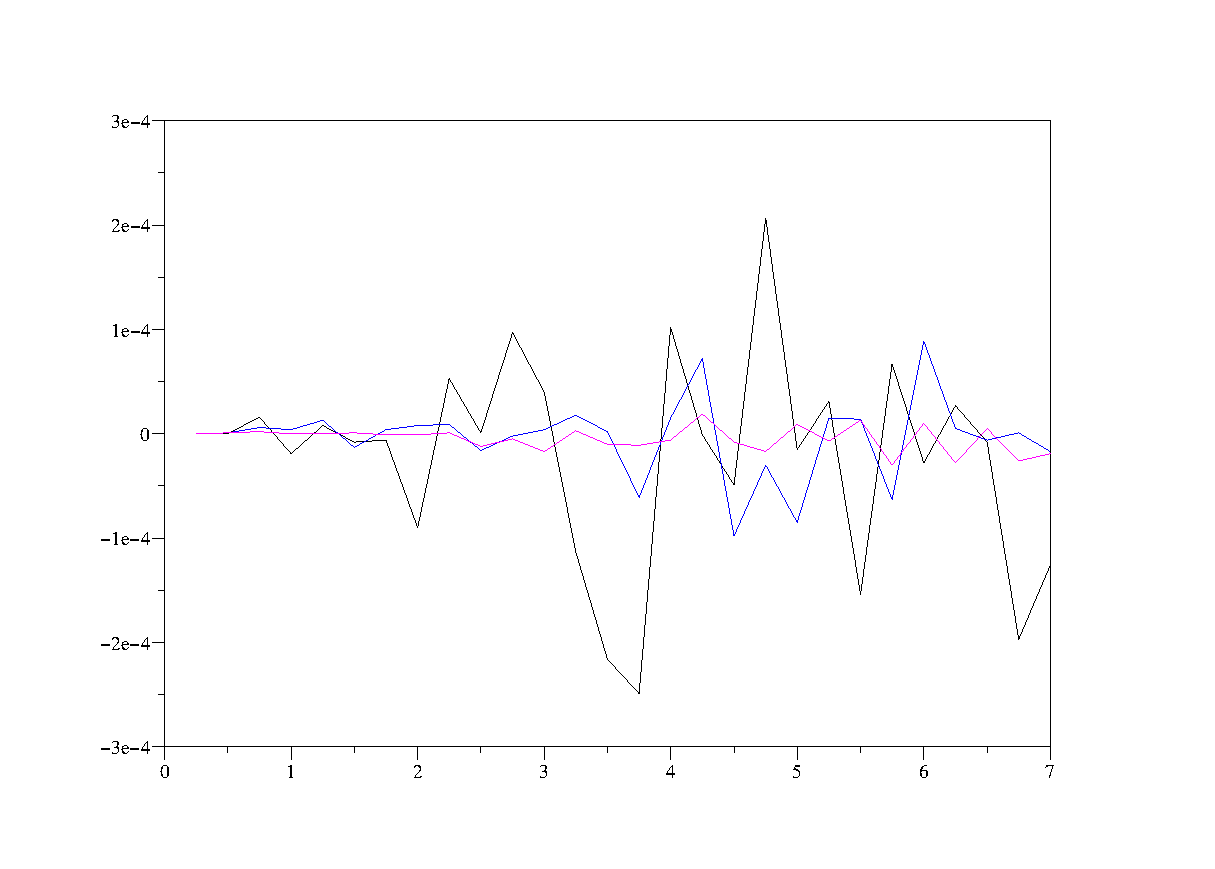
\includegraphics[height=8cm]{./figures/bondserrorY.eps}
\caption{Cumputation bonds error with martingale asset Y for $10 000$, $100 000$ and $1 000 000$ Monte-carlo
  draws, for $\tau=0.25$ and $M=28$ (Number of factor=$1$, $\gamma_i=0.15$ and $L(0,T_i,T_i)=0.05$).}
\label{bonderrorY}
\end{center}
\end{figure}
\begin{figure}[H]
\begin{center}
\includegraphics[height=8cm]{./figures/swptX.eps}
\caption{Swaption prices w.r.t. the time maturity  expiring at $T=7$
  computed with $100 000$ Monte-Carlo draws  with martingale asset X.} 
\label{swptX}
\end{center}
\end{figure}
\begin{figure}[H]
\begin{center}
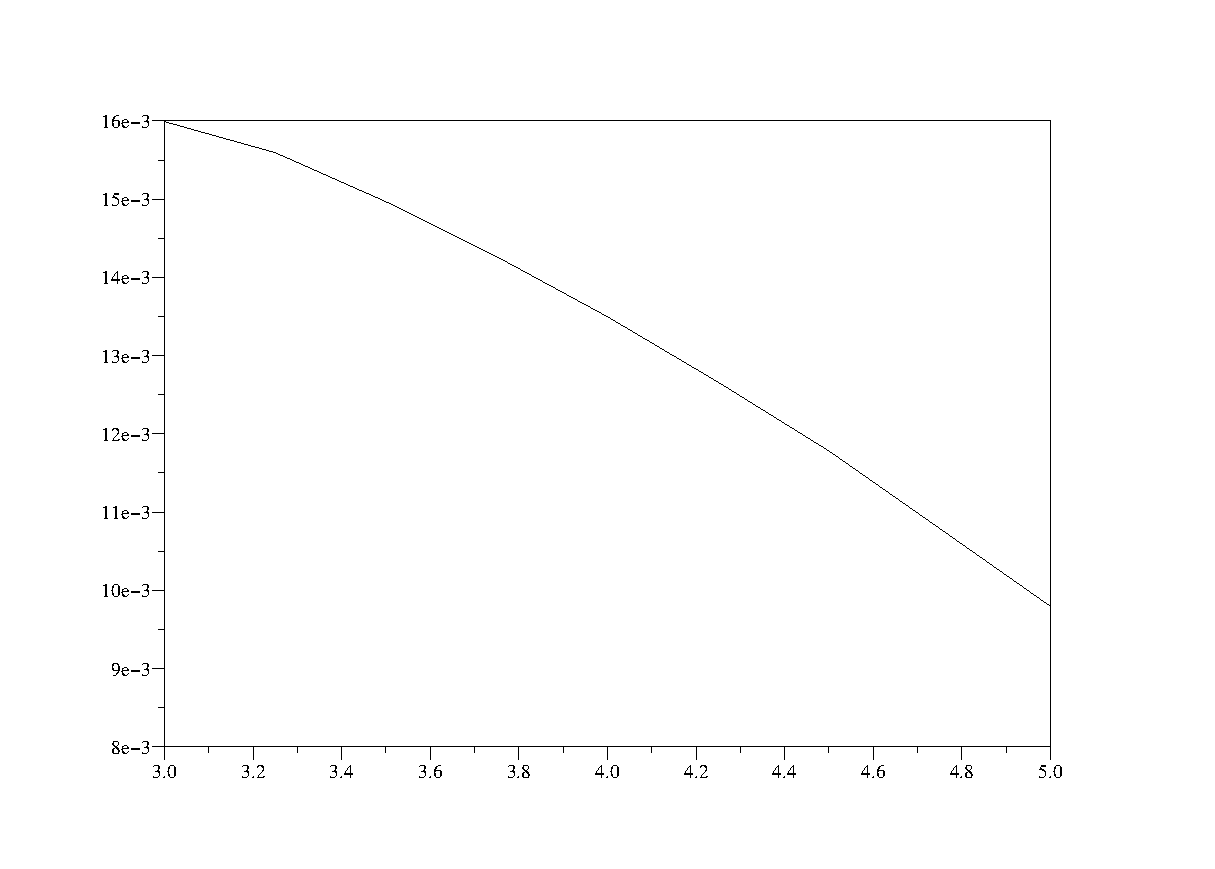
\includegraphics[height=8cm]{./figures/swptY.eps}
\caption{Swaption prices w.r.t. the time maturity  expiring at $T=7$
  computed with $100 000$ Monte-Carlo draws  with martingale asset Y.} 
\label{swptY}
\end{center}
\end{figure}
We can see that the swaption prices simulated with the asset $X$ and the asset $Y$
(for $\tau=0.25$ and $M=28$ Number of factor=$1$, $\gamma_i=0.15$ and
$L(0,T_i,T_i)=0.05$) are very similar with a relative precision of $10^{-2}$.


\subsection{Programming interface}


\subsubsection{C API of the pricer}

Functions name: 
\small{
\begin{verbatim}
int  lmm_caplet_terminalX_pricer(caplets, maturities, numMat, nb_MC, nb_factors, 
                                                           nb_time_step, strike, tenor)

int  lmm_swaption_payer_terminalX_pricer(&swaption_price, swaption_maturity, swap_maturity, 
					          nb_MC, nb_factors, nb_time_step, strike, tenor)

int  lmm_caplet_spotV_pricer( caplets ,  maturities , numMat , nb_MC , nb_factors , 
			                                  nb_time_step , strike ,  tenor);

int lmm_swaption_payer_spotV_pricer(&swaption_price ,  swaption_maturity , swap_maturity   , 
	               			  nb_MC ,  nb_factors ,  nb_time_step ,  strike , tenor);
\end{verbatim}
}

Arguments description:
\begin{itemize}
\item $tenor$ is the period in years of the rate (usually 3 or 6 months); type:double 
\item $numFac$ is the number of factors max 2; type: int
\item $swaption\_maturity$ is the swaption maturity in years; type: double
\item $swap\_maturity$ is the swap maturity in years ; type: double 
\item $strike$ strike of the option; type:double
\item $nb\_MC$ number of monte carlo paths; type: int
\item $nb\_factors$ is the number of factors max 2; type: int
\item $nb\_time\_step$ number of time steps in the euler scheme; type:int 
\end{itemize}


\subsubsection{calling the MartingaleX pricer from a C program}

\small{

\begin{verbatim}
/*************************************************************************************
 *
 *
 *
 *   Example: using Martingale X approach to price caplets and swaptions
 *          
 *
 *  
 *
 *************************************************************************************/
#include<stdio.h>

#include"lmm_martingaleX.h"

int main()
{
  
  double  tenor=0.5;   // period (in years) of the rate usually 3 or 6 months
  int numMat;     
  double *caplets;
  int i;
  double* maturities;
  double swaption_price;
  double swaption_maturity=3;  // swaption maturity in years
  double swap_maturity=7.;     // swap maturity in years
  int nb_MC   =10000;          // number of monte carlo paths
  int nb_time_step=10;         // number of time steps in the euler scheme
  double  strike=0.05;         // strike 
  int nb_factors=2;            // number of factors
  
  
  numMat=(int)(swap_maturity/tenor);
  caplets=(double*)malloc(numMat*sizeof(double));
  maturities=(double*)malloc(numMat*sizeof(double));

  lmm_caplet_terminalX_pricer(caplets, maturities, numMat, nb_MC, nb_factors, 
			      nb_time_step, strike, tenor);
  lmm_swaption_payer_terminalX_pricer(&swaption_price, swaption_maturity, swap_maturity, 
			      nb_MC, nb_factors, nb_time_step, strike, tenor);
  
  for(i=1;i<numMat;i++)
    {
      printf("Caplet(Ti=%lf,%lf,K=%lf)=%lf \n",tenor*i,tenor*i + tenor , strike , caplets[i]);
    }
	
  printf("Swaption price:\n");
  printf("Spt(T=%lf,%lf,K=%lf)=%lf \n",swaption_maturity, swap_maturity, strike, swaption_price);
	
  free(caplets);
  free(maturities);

  return(1);
}


\end{verbatim}

}



we obtain the following result:

\small{

\begin{verbatim}
$ lmm_martingaleX_example 
Caplet prices:
Caplet(Ti=0.500000,1.000000,K=0.050000)=0.003621 
Caplet(Ti=1.000000,1.500000,K=0.050000)=0.004856 
Caplet(Ti=1.500000,2.000000,K=0.050000)=0.005758 
Caplet(Ti=2.000000,2.500000,K=0.050000)=0.006413 
Caplet(Ti=2.500000,3.000000,K=0.050000)=0.006968 
Caplet(Ti=3.000000,3.500000,K=0.050000)=0.007332 
Caplet(Ti=3.500000,4.000000,K=0.050000)=0.007569 
Caplet(Ti=4.000000,4.500000,K=0.050000)=0.007861 
Caplet(Ti=4.500000,5.000000,K=0.050000)=0.008020 
Caplet(Ti=5.000000,5.500000,K=0.050000)=0.008182 
Caplet(Ti=5.500000,6.000000,K=0.050000)=0.008337 
Caplet(Ti=6.000000,6.500000,K=0.050000)=0.008330 
Caplet(Ti=6.500000,7.000000,K=0.050000)=0.008264 
Swaption price:
Spt(T=3.000000,7.000000,K=0.050000)=0.025182 
$ 
\end{verbatim}
}


\subsubsection{calling the MartingaleV pricer from a C program}

\small{

\begin{verbatim}
/**********************************************************************************************
 *
 *
 *
 *   Example: using Martingale V approach to price caplets and swaptions
 *
 *
 *
 *
 *********************************************************************************************/
#include<stdio.h>

#include"lmm_martingaleV.h"


int main()
{


  double  tenor=0.5;   // period (in years) of the rate usually 3 or 6 months
  int numMat;     
  double *caplets;
  int i;
  double* maturities;
  double swaption_price;
  double swaption_maturity=3;  // swaption maturity in years
  double swap_maturity=7.;     // swap maturity in years
  int nb_MC   =10000;          // number of monte carlo paths
  int nb_time_step=10;         // number of time steps in the euler scheme
  double  strike=0.05;         // strike 
  int nb_factors=2;            // number of factors

  
  
  numMat=(int)(swap_maturity/tenor);
  maturities=(double*)malloc((numMat+1)*sizeof(double));
  caplets=(double*)malloc((numMat+1)*sizeof(double));
  lmm_caplet_spotV_pricer( caplets ,  maturities , numMat , nb_MC , nb_factors , 
			   nb_time_step , strike ,  tenor);
  lmm_swaption_payer_spotV_pricer(&swaption_price ,  swaption_maturity , swap_maturity   , 
				  nb_MC ,  nb_factors ,  nb_time_step ,  strike , tenor);

  for(i=1;i<numMat;i++)
    {
      printf("Caplet(Ti=%lf,%lf,K=%lf)=%lf \n", tenor*i ,tenor*(i+1) , strike , caplets[i]);
    }
  printf("Spt(T=%lf,%lf,K=%lf)=%lf \n",swaption_maturity, swap_maturity, strike, swaption_price);
  free(caplets);
  free(maturities);

  return(1);
}

\end{verbatim}

}

we obtain the following result:

\small{

\begin{verbatim}
$ lmm_martingaleV_example 
Caplet(Ti=0.500000,1.000000,K=0.050000)=0.003631 
Caplet(Ti=1.000000,1.500000,K=0.050000)=0.004861 
Caplet(Ti=1.500000,2.000000,K=0.050000)=0.005767 
Caplet(Ti=2.000000,2.500000,K=0.050000)=0.006418 
Caplet(Ti=2.500000,3.000000,K=0.050000)=0.006967 
Caplet(Ti=3.000000,3.500000,K=0.050000)=0.007347 
Caplet(Ti=3.500000,4.000000,K=0.050000)=0.007592 
Caplet(Ti=4.000000,4.500000,K=0.050000)=0.007895 
Caplet(Ti=4.500000,5.000000,K=0.050000)=0.008064 
Caplet(Ti=5.000000,5.500000,K=0.050000)=0.008215 
Caplet(Ti=5.500000,6.000000,K=0.050000)=0.008379 
Caplet(Ti=6.000000,6.500000,K=0.050000)=0.008381 
Caplet(Ti=6.500000,7.000000,K=0.050000)=0.008326 
Spt(T=3.000000,7.000000,K=0.050000)=0.025197 
$ 
\end{verbatim}
}


\subsubsection{A Scilab function for the MartingaleX and MartingaleV pricers}

The scilab functions are given below:


\small{
\begin{verbatim}
lmm_cap_martX_sci(period , nb_fac , maturity , strike )
lmm_swpt_martX_sci(period , nb_fac , swpt_maturity , swp_maturity , strike )
lmm_cap_spotV_sci(period , nb_fac , maturity , strike )
lmm_swpt_spotV_sci(period , nb_fac , swpt_maturity , swp_maturity , strike )
\end{verbatim} 
}

they can be found in the file lmm\_scilab.sci,  they return the price of the options  and the input parameters are 

\begin{itemize}
\item {\it period} is the period length of the rate; type:double
\item {\it nb\_fac} is the number of factors; type: int
\item {\it maturity} is the maturity used to price all caplets; type: double
\item {\it swpt\_mat} is the swpation maturity in years; type: double
\item {\it swp\_mat} is th swap maturity in years; type: double
\item {\it strike} the strike; type: double
\end{itemize}


{\bf Loading the scilab functions}: first you should compile the library, report to the README file. At the scilab ``File'' menu click on ``File Operations'' then select the file ``lmm\_scilab.sci'' and click on ``Getf'' buttom, it will produce something like this in ``scilex''
\small{
\begin{verbatim} 
-->;getf("/home/der_mif/jose/recherche/taux/prog/cprog/bgmPremia/code/lmm_scilab.sci");
\end{verbatim} 
}

all functions within this file are now available at the prompt or can be called from a scilab program. 
 
We illustrate the use of the above functions: 

We obtained the following result from scilab-2.7:

\small{
\begin{verbatim}
-->b=lmm_cap_martX_sci(0.5 , 2 , 7 , 0.05)                                       
shared archive loaded
Link done
 b  =
 
!   0.           0.  !
!   0.0036211    0.5 !
!   0.0048560    1.  !
!   0.0057583    1.5 !
!   0.0064130    2.  !
!   0.0069682    2.5 !
!   0.0073320    3.  !
!   0.0075693    3.5 !
!   0.0078611    4.  !
!   0.0080204    4.5 !
!   0.0081819    5.  !
!   0.0083375    5.5 !
!   0.0083296    6.  !
!   0.0082636    6.5 !
 
-->
\end{verbatim} 
}

\small{
\begin{verbatim}
 
-->b=lmm_swpt_martX_sci(0.5,2,3,7,0.05)
shared archive loaded
Link done
 b  =
 
    0.0251820  
 
-->
\end{verbatim} 
}


\small{
\begin{verbatim}

-->b=lmm_swpt_spotV_sci(0.5,2,3,7,0.05)
shared archive loaded
Link done
 b  =
 
    0.0251971   
-->
\end{verbatim} 
}

The $lmm_cap_spotV_sci$ function leads to failure of the scilab program, we suggest not to use it. 


